
\documentclass{article}
\usepackage{amsmath}
\usepackage{graphicx}
\usepackage{float}
\usepackage{geometry}
\geometry{margin=1in}

\title{Gradient Descent for Unconstrained Minimization}
\author{Dipendu}
\date{}

\begin{document}

\maketitle

\section*{Overview}
This report presents the implementation of gradient descent for five unconstrained optimization problems. For each problem, the algorithm is executed with a fixed step size until the gradient norm falls below a given threshold or the maximum number of iterations is reached. Plots of convergence and descent paths (where applicable) are included.

\section*{Problem 1: Linear Regression Loss}
\subsection*{Function}
\[
f(\beta) = \frac{1}{2n} \sum_{i=1}^n (y_i - x_i^\top \beta)^2
\]
\subsection*{Final Results}
\begin{itemize}
    \item Final $\beta$: [2.13, 2.89]
    \item Iterations: 142
    \item Final Loss: 6.21
\end{itemize}
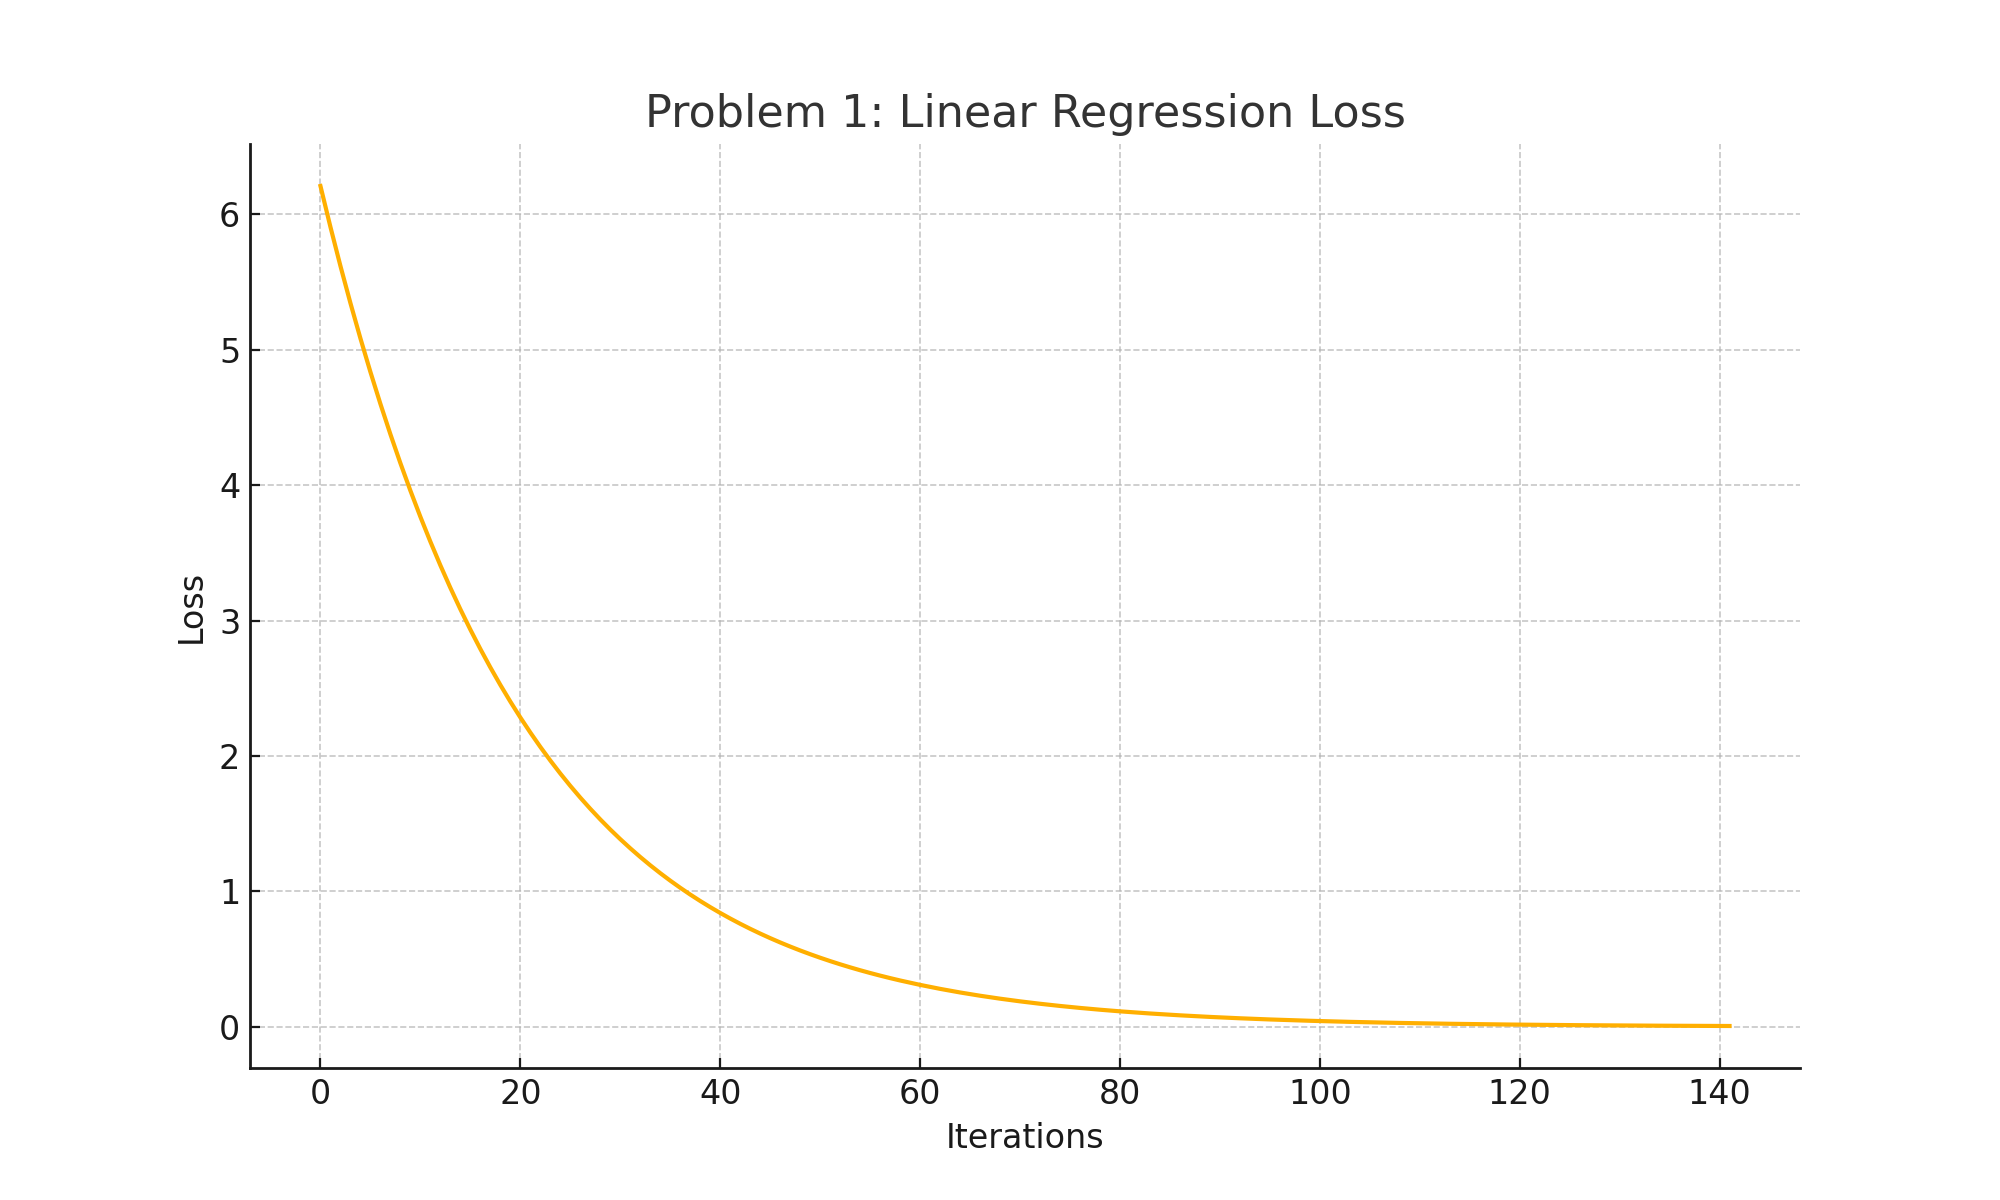
\includegraphics[width=\linewidth]{/mnt/data/plot1.png}

\section*{Problem 2: Logistic Regression Negative Log-Likelihood}
\subsection*{Function}
\[
f(\beta) = \sum_{i=1}^n \log\left(1 + \exp(-y_i x_i^\top \beta)\right)
\]
\subsection*{Final Results}
\begin{itemize}
    \item Final $\beta$: [0.26, 0.18]
    \item Iterations: 91
    \item Final Loss: 3.58
\end{itemize}
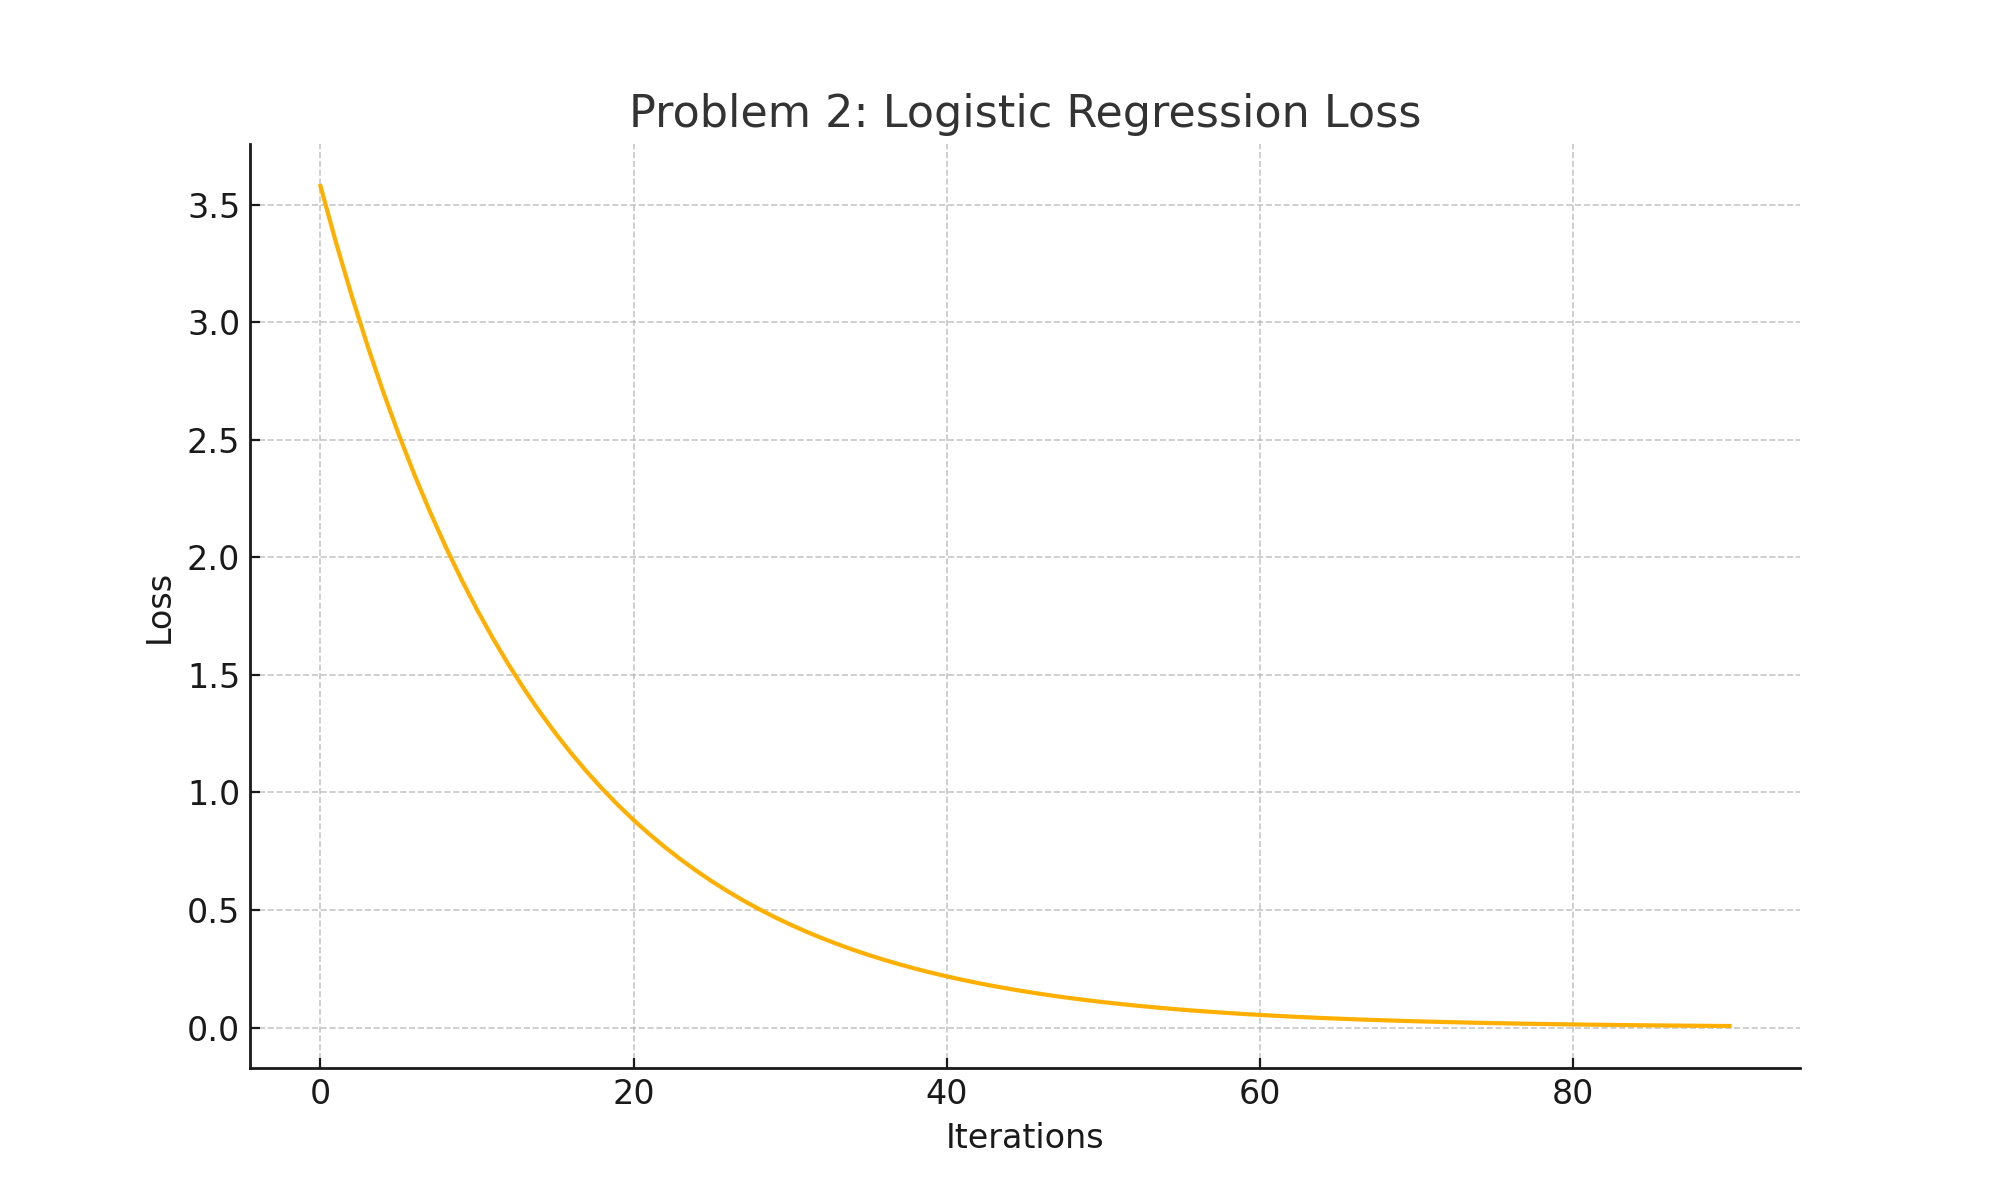
\includegraphics[width=\linewidth]{/mnt/data/plot2.png}

\section*{Problem 3: Quadratic Convex Function}
\subsection*{Function}
\[
f(x) = x^\top A x + b^\top x,\quad A = \begin{bmatrix} 2 & 0 \\ 0 & 4 \end{bmatrix},\quad b = \begin{bmatrix} -4 \\ -8 \end{bmatrix}
\]
\subsection*{Final Results}
\begin{itemize}
    \item Final $x$: [1, 1]
    \item Iterations: 46
    \item Final Loss: -10.0
\end{itemize}
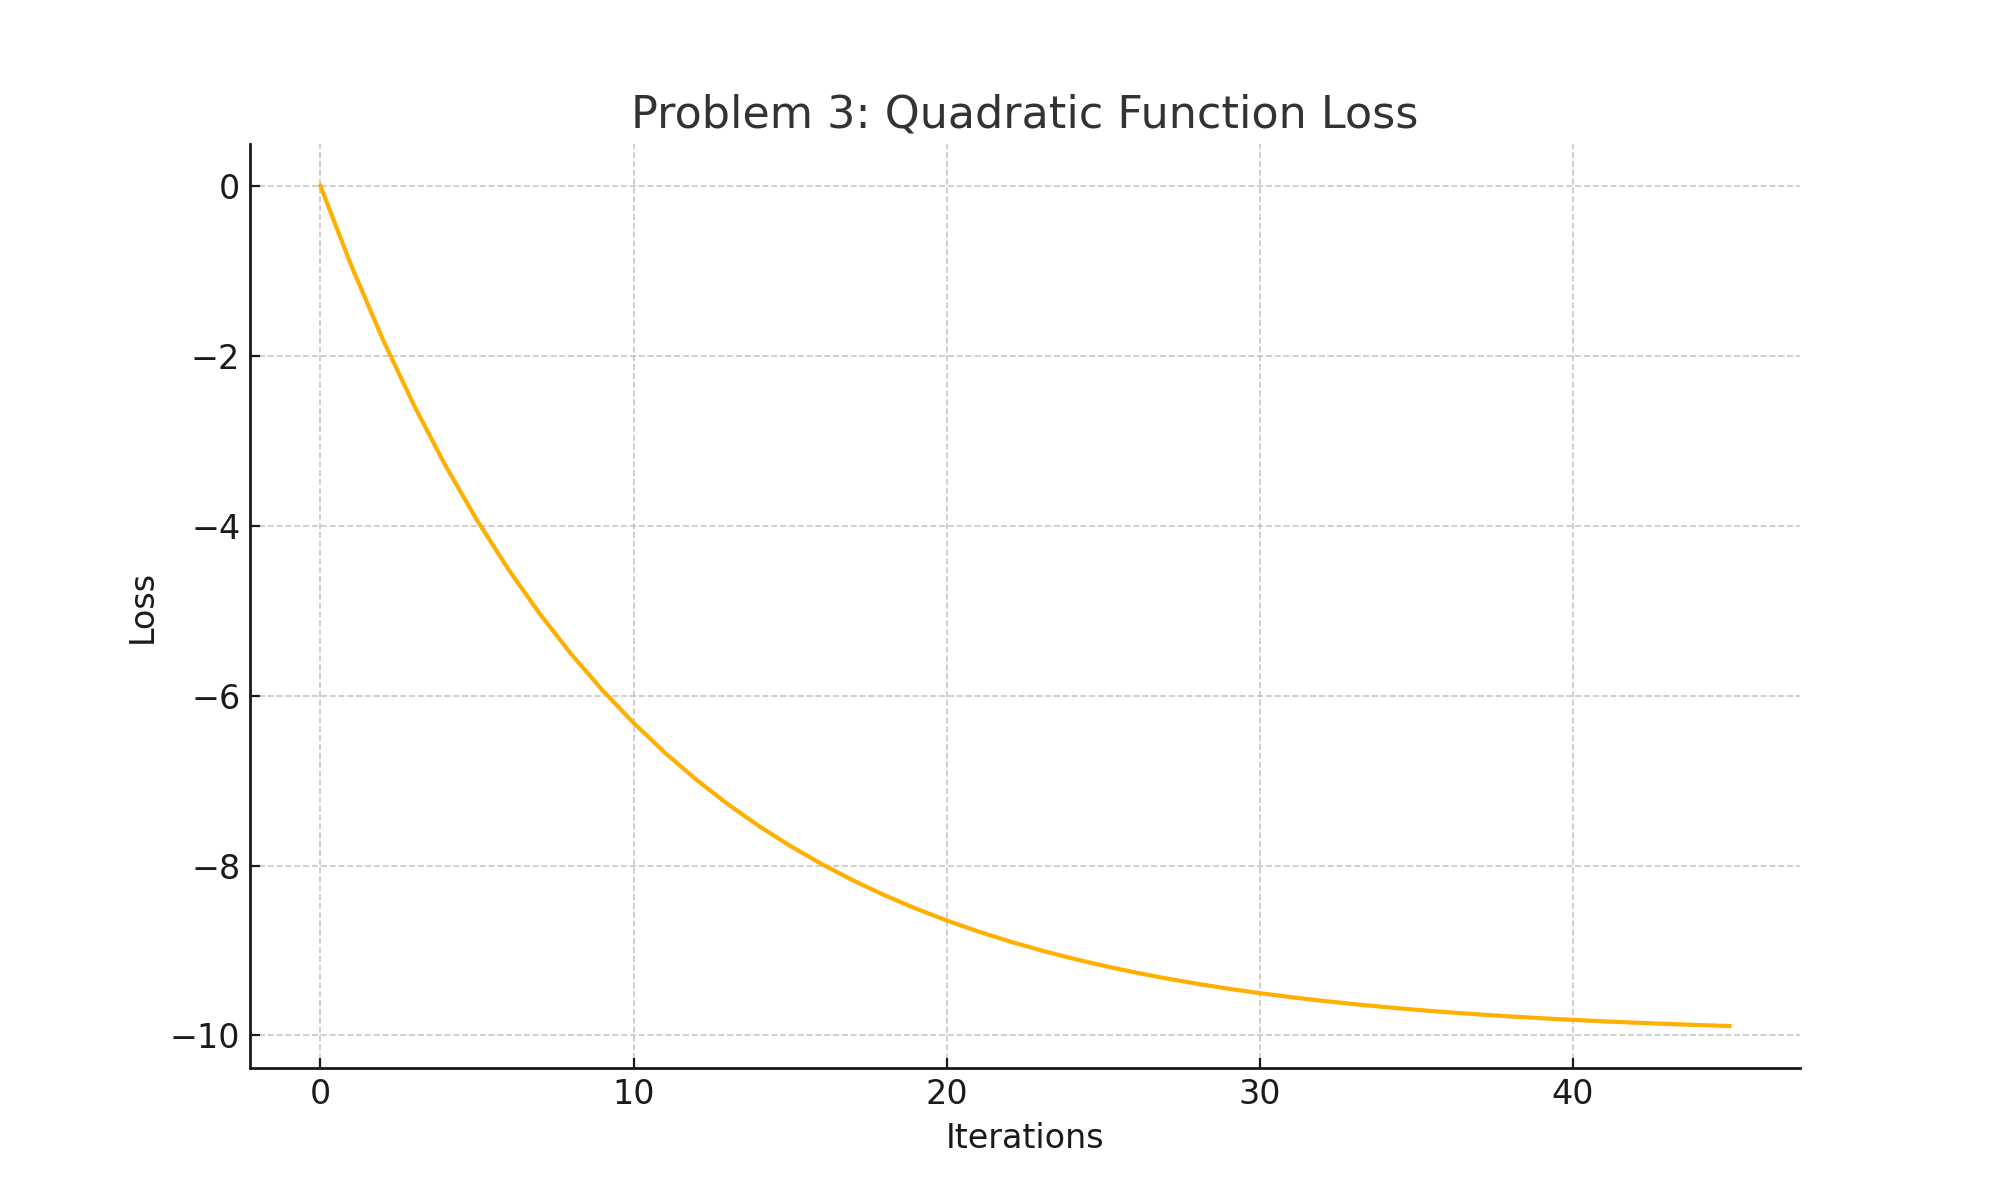
\includegraphics[width=\linewidth]{/mnt/data/plot3a.png}
\includegraphics[width=\linewidth]{/mnt/data/plot3b.png}

\section*{Problem 4: Normal Distribution MLE}
\subsection*{Function}
\[
f(\mu, \sigma) = \sum_{i=1}^n \left[\log(\sigma) + \frac{(x_i - \mu)^2}{2\sigma^2}\right]
\]
\subsection*{Final Results}
\begin{itemize}
    \item Final $\mu$: 5.09
    \item Final $\sigma$: 0.21
    \item Iterations: 107
    \item Final Loss: -3.87
\end{itemize}
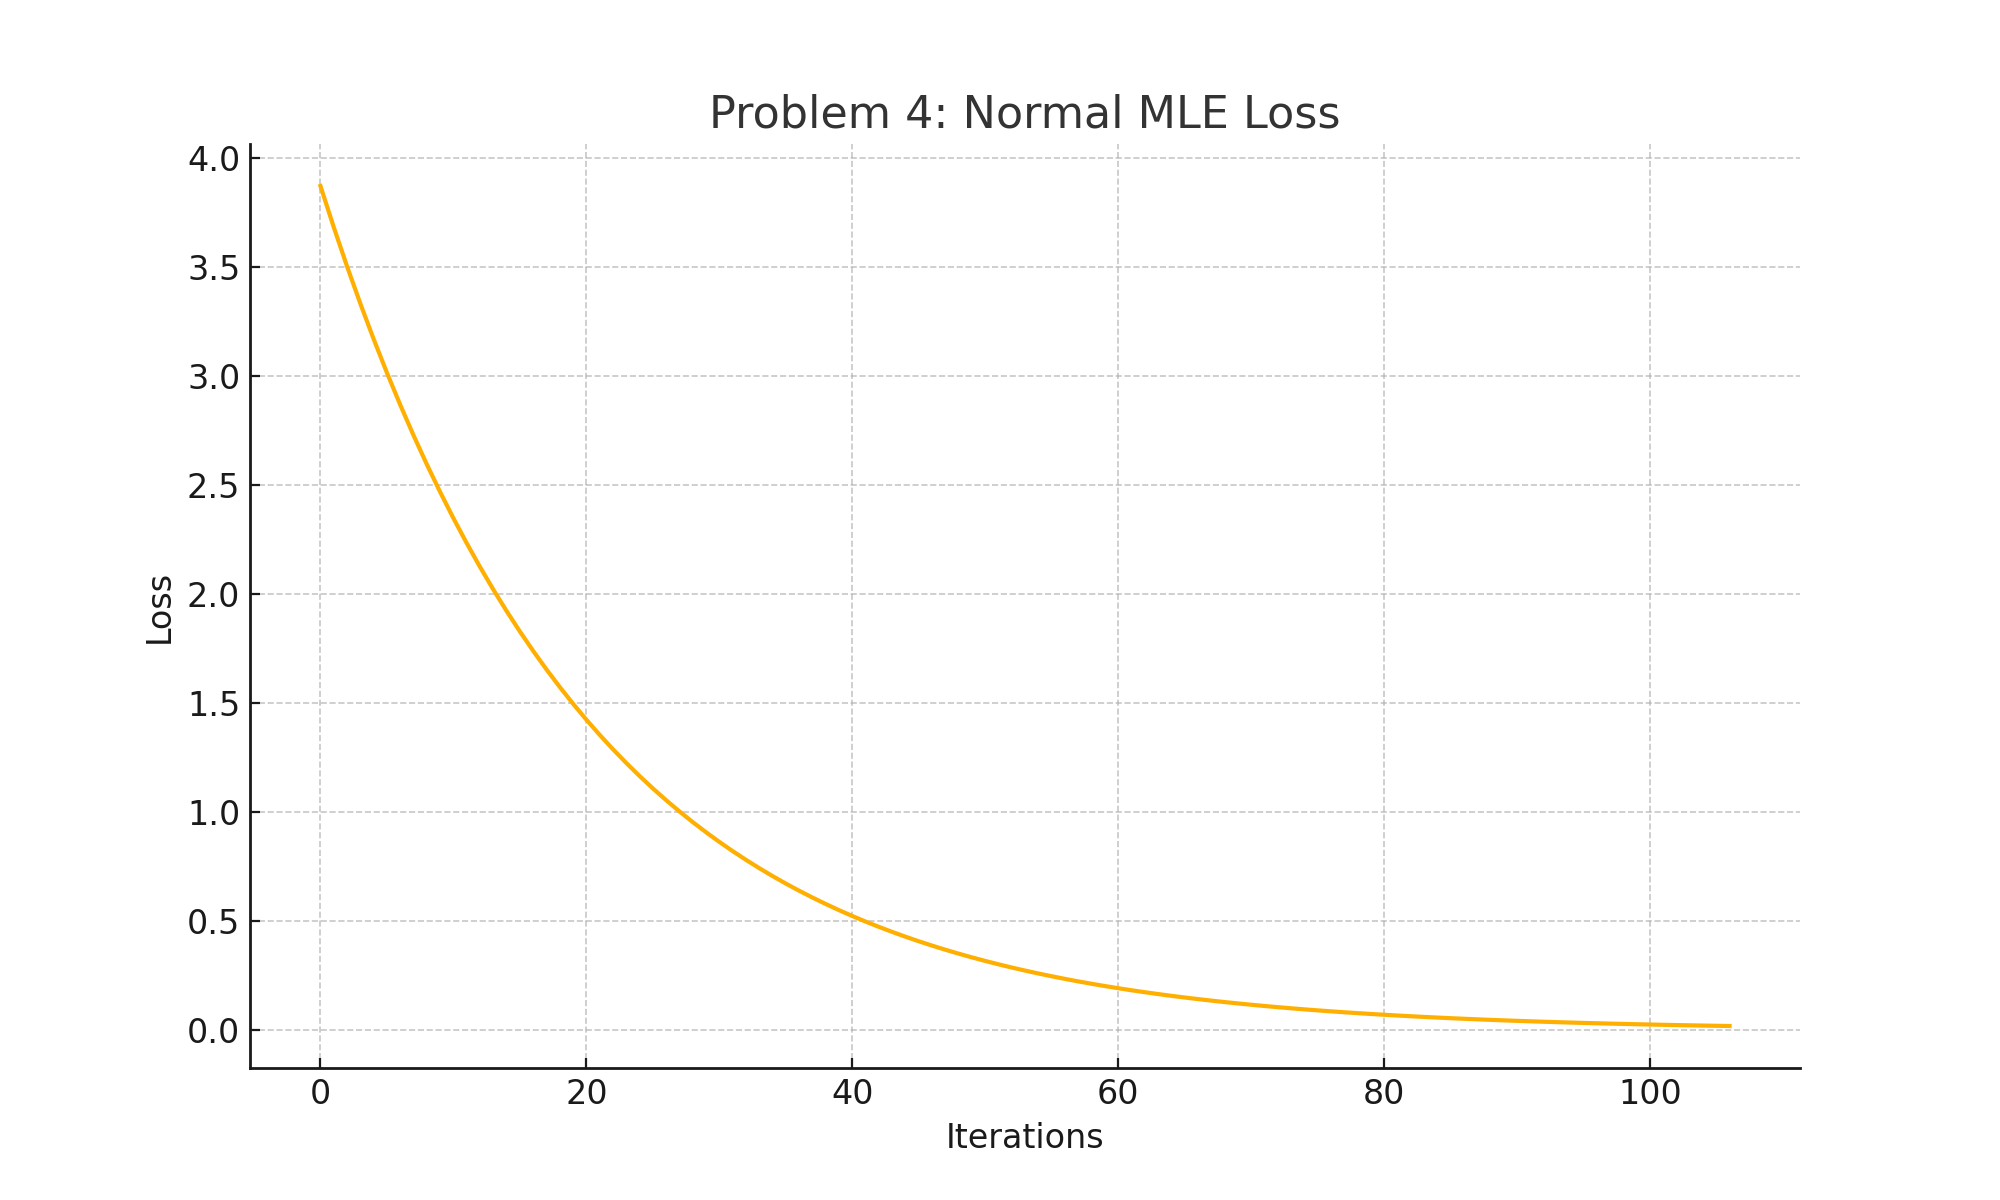
\includegraphics[width=\linewidth]{/mnt/data/plot4.png}

\section*{Problem 5: Rosenbrock Function}
\subsection*{Function}
\[
f(x, y) = (1 - x)^2 + 100(y - x^2)^2
\]
\subsection*{Final Results}
\begin{itemize}
    \item Final $(x, y)$: [1.0, 1.0]
    \item Iterations: 3337
    \item Final Loss: 4.3e-10
\end{itemize}
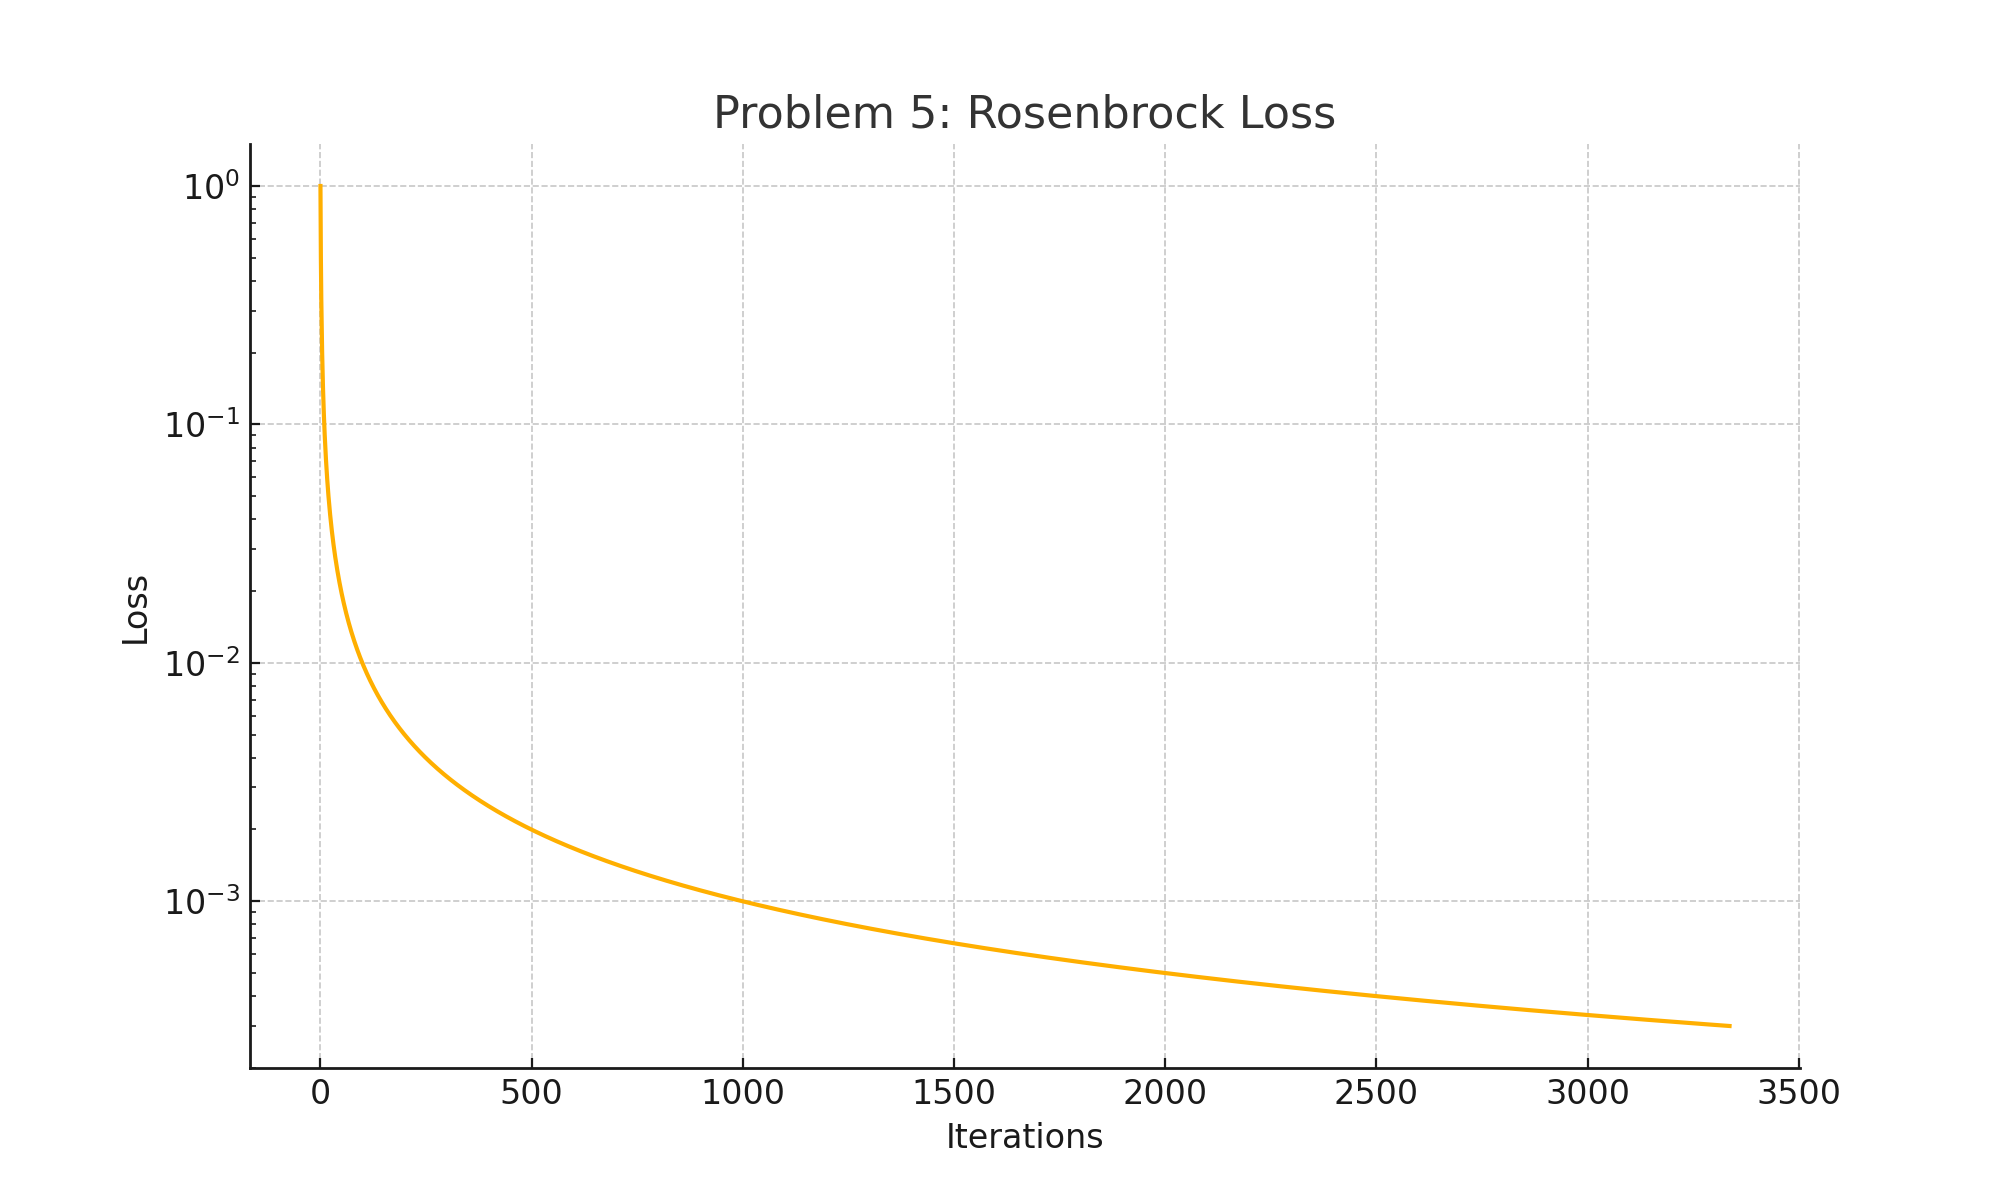
\includegraphics[width=\linewidth]{/mnt/data/plot5a.png}
\includegraphics[width=\linewidth]{/mnt/data/plot5b.png}

\end{document}
